\documentclass{article}
\usepackage{graphicx}
\usepackage{wrapfig}
\usepackage{filecontents}
\usepackage{siunitx}
\usepackage[table]{xcolor}
\usepackage{float}
\usepackage{hyperref}

\usepackage{color} % balíček pro obarvování textů
\usepackage{xcolor}  % zapne možnost používání barev, mj. pro \definecolor
\usepackage{pgfplots} % http://www.chiark.greenend.org.uk/doc/texlive-doc/latex/pgfplots/pgfplots.pdf

\ifnum 0\ifxetex 1\fi\ifluatex 1\fi=0 % if pdftex
  \usepackage[T1]{fontenc}
  \usepackage[utf8]{inputenc}
\else % if luatex or xelatex
  \ifxetex
    \usepackage{mathspec}
  \else
    \usepackage{fontspec}
  \fi
  \defaultfontfeatures{Ligatures=TeX,Scale=MatchLowercase}
\fi
\usepackage[total={175mm,230mm}, top=23mm, left=20mm, includefoot]{geometry}
\hypersetup{
    colorlinks,
    linkcolor={blue!50!black},
    citecolor={green!50!black},
    urlcolor={blue!80!black}
}
\definecolor{orange}{RGB}{ 251, 114, 032}
\definecolor{fialova}{RGB}{ 255, 000, 255}

\newcounter{obrazky}
\setcounter{obrazky}{1}
\newcommand \obrlabel[1]
{ 
  obr.~\theobrazky
  \stepcounter{obrazky}
  \label{#1}
}


\newcommand \obr[1]
{ obr.~\ref{#1}}

\newcommand \tab[1]
{ tab.~\ref{#1}}


\begin{document}
\section{Ověřování základních vlastností OZ}
Budeme pracovat s OZ 1458:
\begin{itemize}
  \item Stejnosměrné zesílení: \(A_0 \approx  200000\) (ideálně \(\infty \)).
  \item Vstupní odpor: \(R_{in} \approx 1\-[M\Omega]\) (ideálně \(\infty \)).
  \item Výstupní odpor: \(R_{out} \approx 75\-[\Omega]\) (ideálně \(0\)).
  \item Rozsah výstupního napětí: od \(-U_{SAT}\) do \(+U_{SAT}\), \(U_{SAT} \approx U_{napájecí}\) \(-(1 2)\-[V]\).
\end{itemize}
\subsection*{Dynamické vlastnosti OZ} 
\begin{figure}[H]
  \begin{minipage}[t]{0.49\textwidth}
    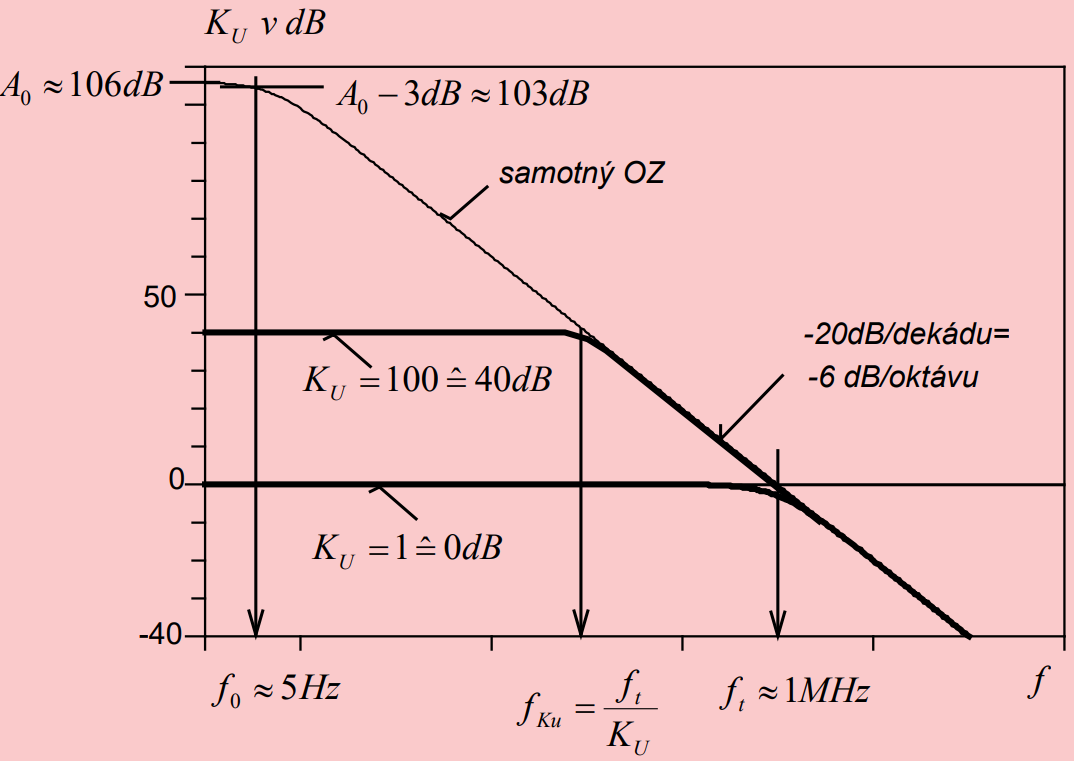
\includegraphics[width=\textwidth]{priprava/sirka_pasma.png}
    % \centering{\obrlabel{sirka_pasma}}
  \end{minipage}
  \hfill
  \begin{minipage}[t]{0.49\textwidth}
    \vspace{-0.6\textwidth}
    U OZ 1458 dochází při plném zesílení \(A_0\) k jeho poklesu o \(3\-[dB]\) už u frekvence \( F_0 \approx 5\-[Hz]\) a tranzitní kmitočet \(F_t \approx 1\-[MHz]\).
    Tranzitní kmitočet \(F_t\) je frekvence, při které dochází k poklesu zesílení na \(0\-[dB]\) neboli zesílení \(1\).
    Zhruba platí empirický vztah \\
    \\
    \(A_0 \cdot F_{Ku} = F_t\) \\
    \\
    kde \(F_{Ku}\) je kmitočet při daném zesílení, na kterém dochází k poklesu zesílení o \(3\-[dB]\).
  \end{minipage}
\end{figure}

\begin{figure}[H]
  \begin{minipage}[t]{0.49\textwidth}
    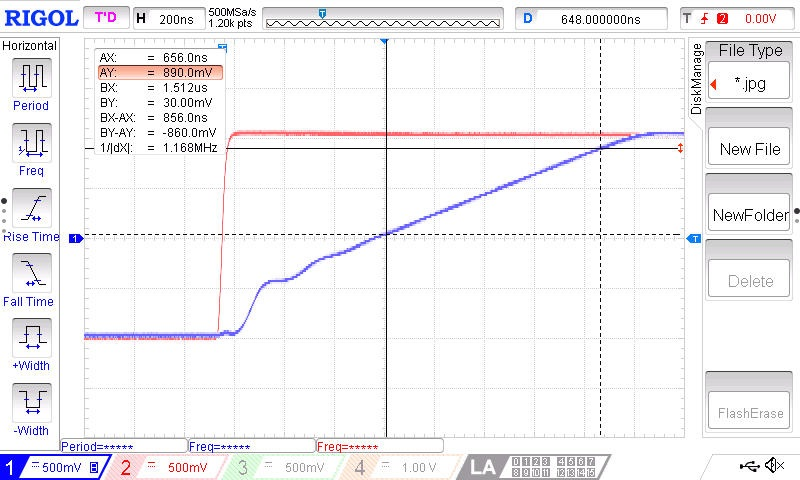
\includegraphics[width=\textwidth]{LAB/NewFile02.jpg}
    % \centering{\obrlabelmereni_SR}}
  \end{minipage}
  \hfill
  \begin{minipage}[t]{0.49\textwidth}
    \vspace{-0.5\textwidth}
    Další důležitý parametr je mezní rychlost přeběhu neboli Slew rate \(SR\), který udává maximální strmost výstupní hrany.
    Jde tedy o jednotky \(V/s\), ale většinou se z praktických důvodů používá \(V/\mu s\) a u OZ 1458 je \(SR \approx 0.5\-[V/\mu s]\).
    Platí tedy \(SR = \frac{\Delta_u}{\Delta_t}\) a měření lze realizovat pomocí osciloskopu a obdélníkového signálu na vstupu zesilovače.
    Jak je vidět na \obr{mereni_SR}, je potřebné neměřit strmost hrany od jejího začátku po konec, protože by bylo měření zkreslené přechodovými ději.
  \end{minipage}
\end{figure}  

\section*{Simulované proudy a napětí v obvodech}
\subsection*{Sledovač}
\begin{figure}[H]
  \centering
  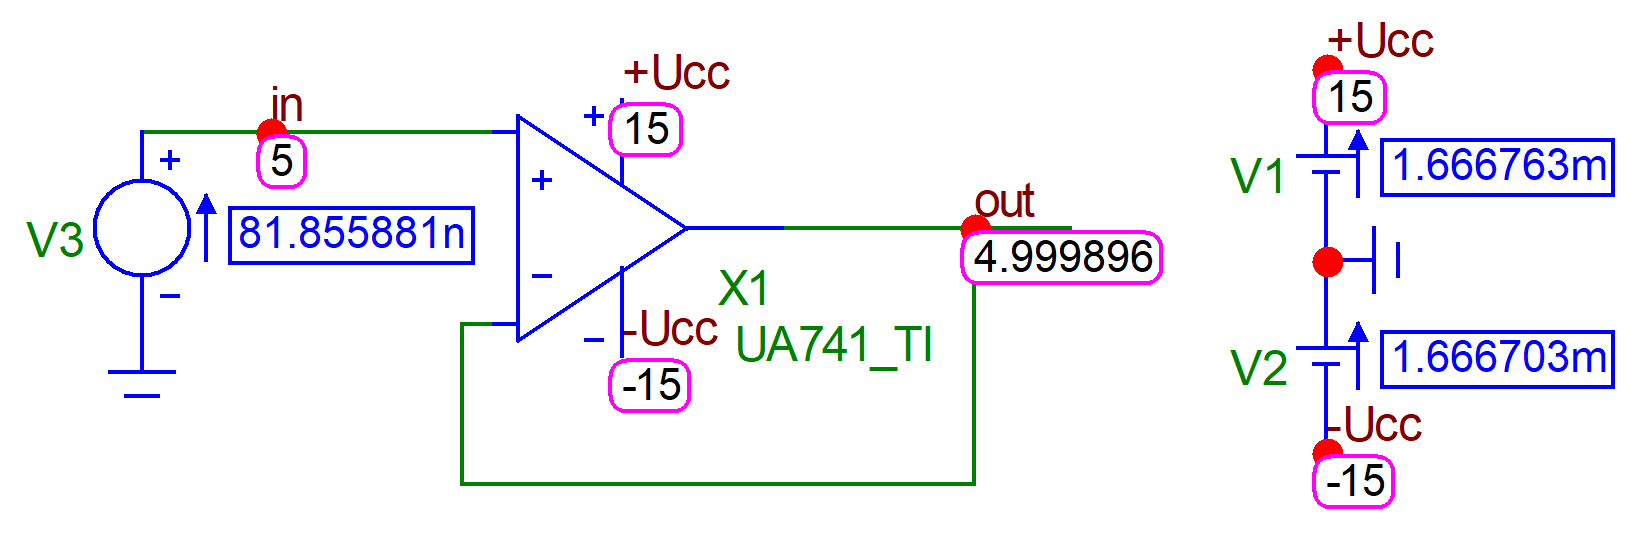
\includegraphics[width=0.48\textwidth]{PC/Dynamic_DC/sledovač.png}
\end{figure}

\begin{figure}[H]
  \begin{minipage}[t]{0.48\textwidth}
    \subsection*{Invertující zesilovač}
    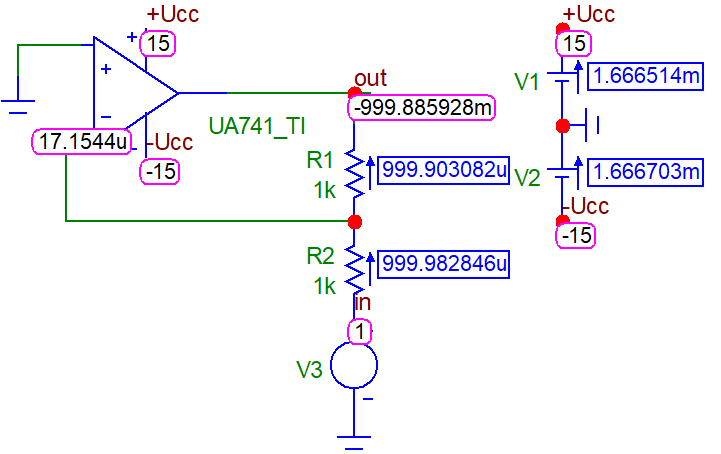
\includegraphics[width=\textwidth]{PC/Dynamic_DC/in.png}
  \end{minipage}
  \hfill
  \begin{minipage}[t]{0.48\textwidth}
    % \vspace{-0.5\textwidth}
    \subsection*{Neinvertující zesilovač}
    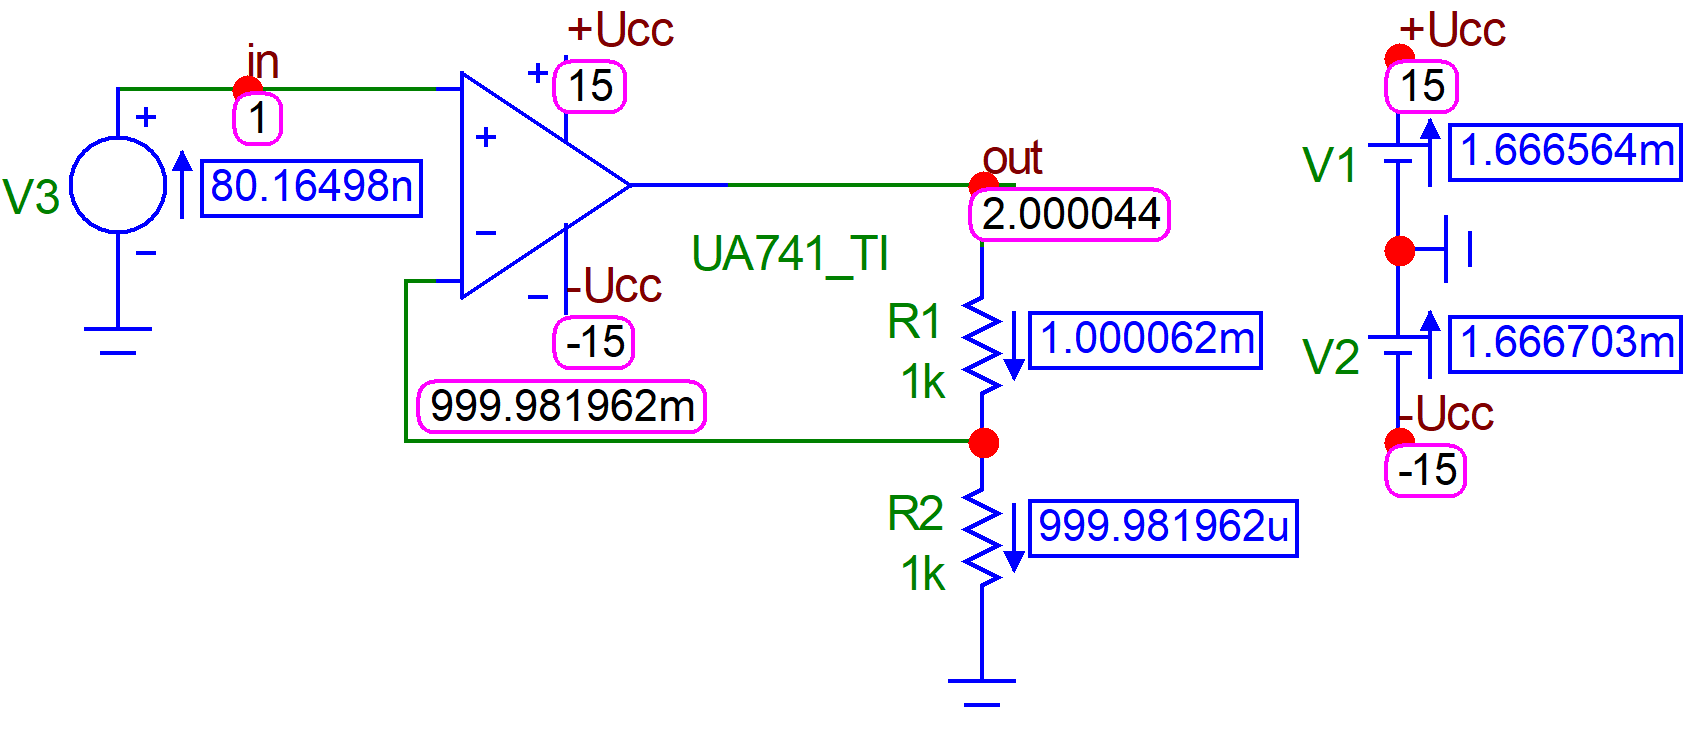
\includegraphics[width=\textwidth]{PC/Dynamic_DC/nein.png}
  \end{minipage}
\end{figure}

\section*{Rychlost Přeběhu}
\begin{figure}[H]
  \begin{minipage}[t]{0.5\textwidth}
    \subsection*{Simulace}
    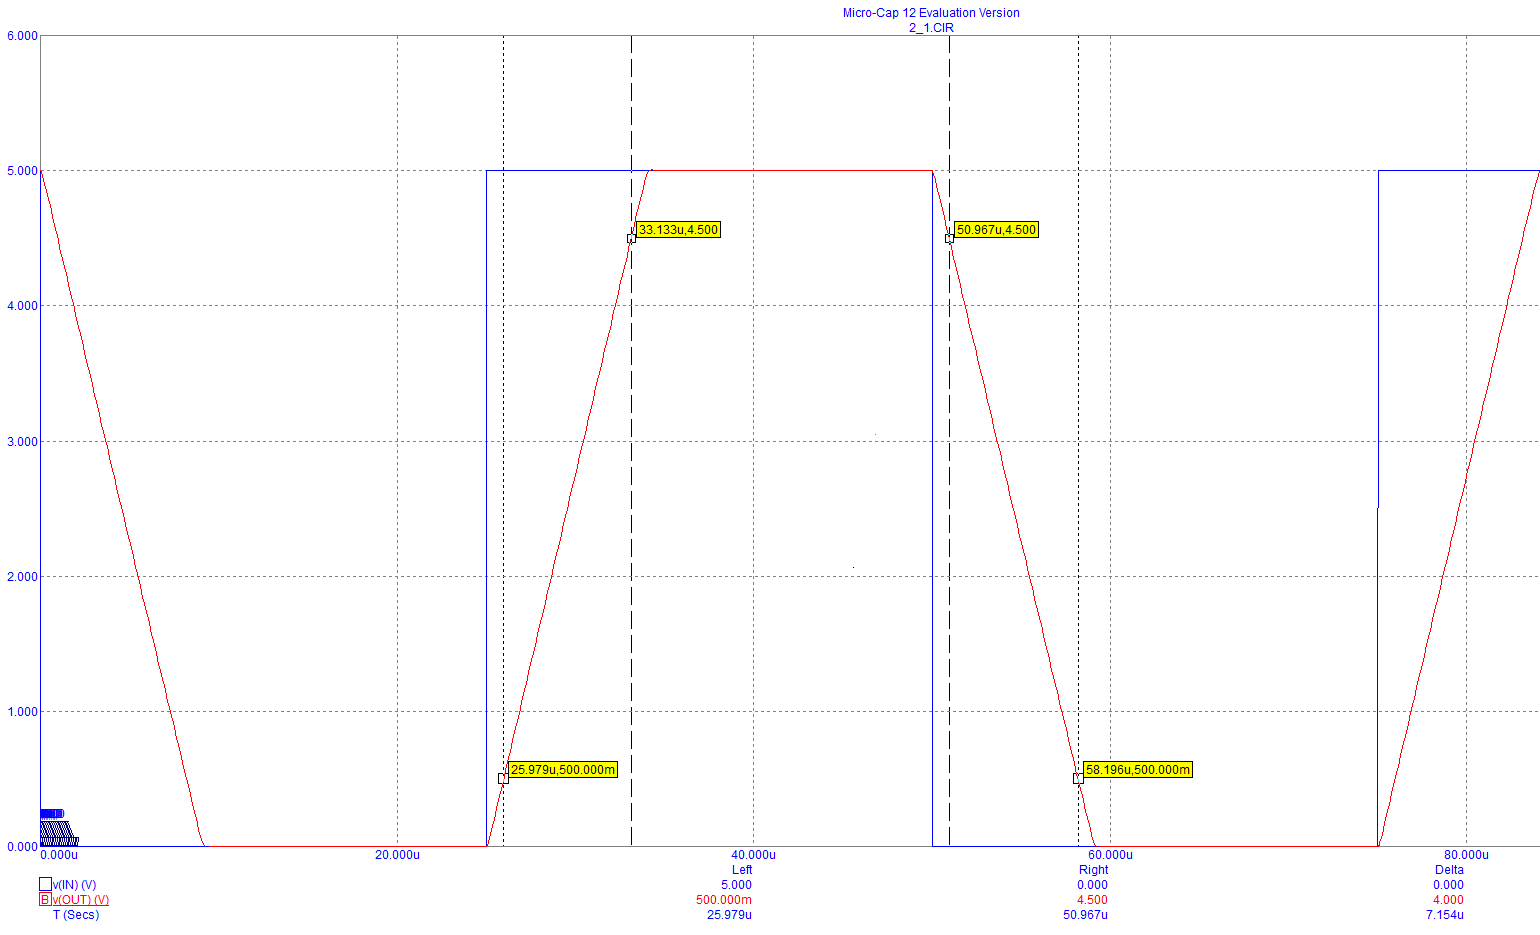
\includegraphics[width=\textwidth]{PC/Tranzientni/rychlost_prebehu.png}
  \end{minipage}
  \hfill
  \begin{minipage}[t]{0.5\textwidth}
    % \vspace{-3mm}
    \subsection*{Reálné měření}
    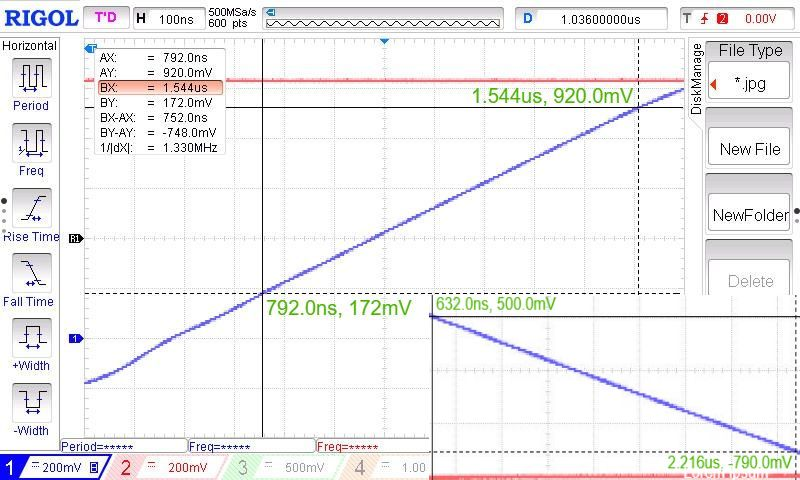
\includegraphics[width=\textwidth]{LAB/NewFile03.jpg}
  \end{minipage}
% \end{figure}
\vspace{5mm}
% \begin{figure}[H]
  \begin{minipage}[t]{0.5\textwidth}
    \(
      SR_{up} = \frac{\Delta_u}{\Delta_t} = \frac{U_2-U_1}{t_2-t_1} = \frac{4.5-0.5}{(33.133-25.979)\cdot 10^{-6}} =\\= 559128\-[V/s] = 0.559128\-[V/\mu s]
    \) 
  \end{minipage}
  \hfill
  \begin{minipage}[t]{0.5\textwidth}
    \(
      SR_{up} = \frac{\Delta_u}{\Delta_t} = \frac{U_2-U_1}{t_2-t_1} = \frac{0.920-0.172}{1.544\cdot 10^{-6}-792\cdot 10^{-9}} =\\= 994680\-[V/s] = 0.994680\-[V/\mu s]
    \) 
  \end{minipage}
% \end{figure}
\vspace{5mm}
% \begin{figure}[H]
  \begin{minipage}[t]{0.5\textwidth}
    \(
      SR_{down} = \frac{\Delta_u}{\Delta_t} = \frac{U_2-U_1}{t_2-t_1} = \frac{0.5-4.5}{(58.196-50.967)\cdot 10^{-6}} =\\= -553327\-[V/s] = -0.553327\-[V/\mu s]
    \)
  \end{minipage}
  \hfill
  \begin{minipage}[t]{0.5\textwidth}
    \(
      SR_{down} = \frac{\Delta_u}{\Delta_t} = \frac{U_2-U_1}{t_2-t_1} = \frac{-0.79-0.5}{2.216\cdot 10^{-6}-632\cdot 10^{-9}} =\\= -814394\-[V/s] = -0.814394\-[V/\mu s]
    \)
  \end{minipage}
\end{figure}

\section*{Základní časové průběhy}
\begin{figure}[H]
  \begin{minipage}[t]{0.38\textwidth}
    \subsection*{Neinvertující zesilovač}
    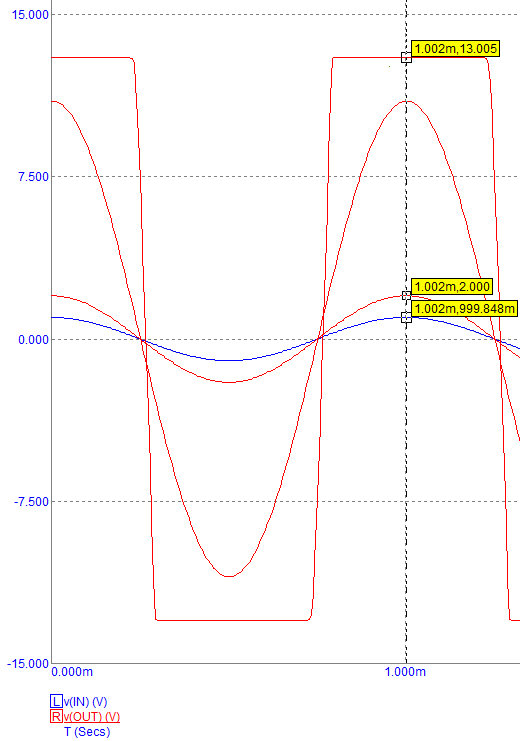
\includegraphics[width=\textwidth]{PC/Tranzientni/nein.png}
  \end{minipage}
  \hfill
  \begin{minipage}[t]{0.32\textwidth}
    % \vspace{-0.5\textwidth}
    \subsection*{Invertující zesilovač}
    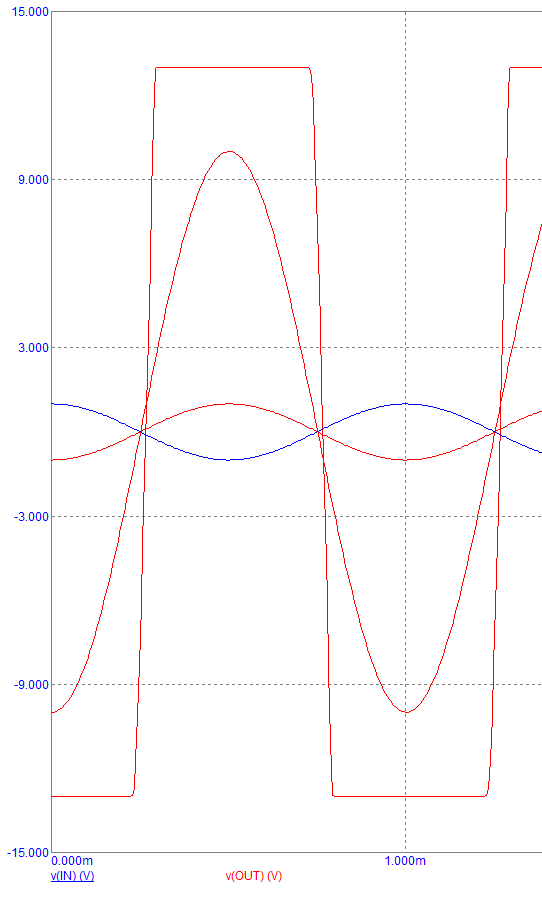
\includegraphics[width=\textwidth]{PC/Tranzientni/in.png}
  \end{minipage}
  \hfill
  \begin{minipage}[t]{0.25\textwidth}
    Reálné změřené časové průběhy jsou níže na \obr{sin_prubehy}. 

    Tři výstupní průběhy se odlišují hodnotami odporu \(R_1 = (1, 10, 100\-[k\Omega])\) zatím co \(R_2 = 1\-[k\Omega]\) zůstává stejný.
    Zesílení tak teoreticky dosahuje hodnot \\\(|A_0| = (2, 11, 101)\) což je pravda dokud nedojde k saturaci.
  \end{minipage}
  \begin{figure}[H]
    \begin{minipage}[t]{0.49\textwidth}
      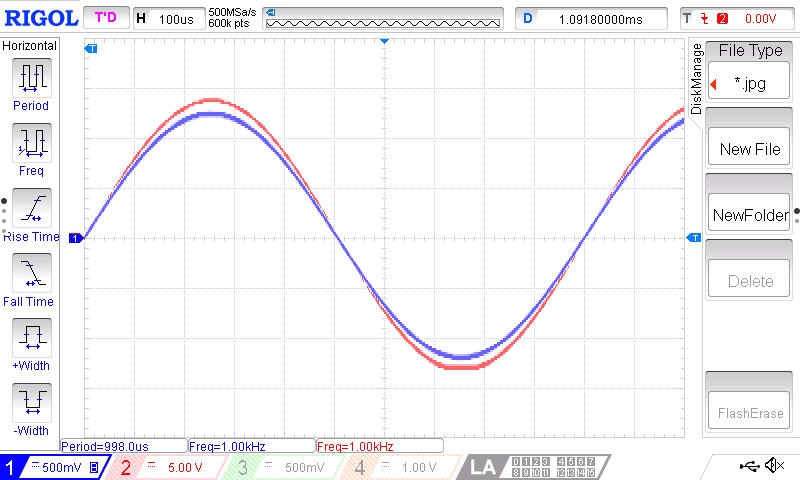
\includegraphics[width=\textwidth]{LAB/NewFile11.jpg}
      \center{A}\\
      \vspace{1mm}
      \(f = 1\-[kHz]\), \(U_(ss-in) = 2.06\-[V]\), \(U_(ss-out) = 28.6\-[V]\)\\
      \(A = \frac{U_(ss-out)}{U_(ss-in)} = \frac{28.6}{2.06} = 13.88\-[-]\)
    \end{minipage}
    \hfill
    \begin{minipage}[t]{0.49\textwidth}
      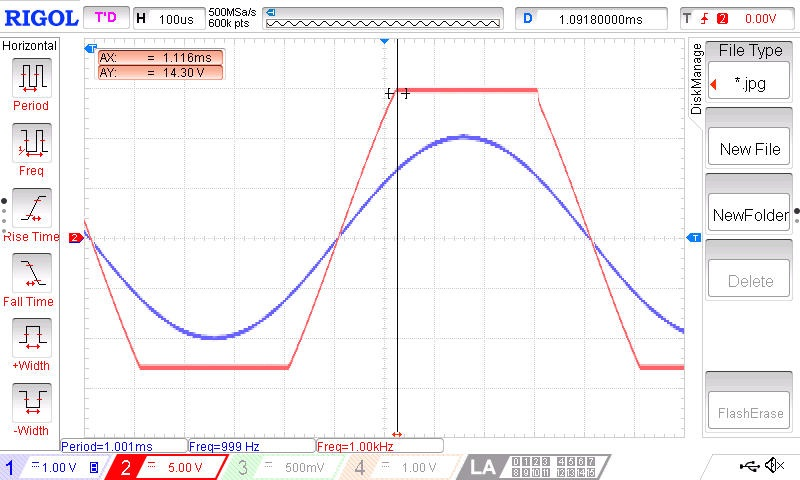
\includegraphics[width=\textwidth]{LAB/NewFile08.jpg}
      \center{B}\\
      \vspace{1mm}
      \(1\-[kHz]\), \(U_(ss-in) = 4\-[V]\), \(U_(ss-out) = 28\-[V]\)\\
      Pokud by nedošlo k saturaci, tak by zesílení \(A\) mělo být stejné jako na průběhu vedle \(A = 13.59\-[V]\).
      Jediná změna mezi těmito průběhy je totiž amplitudová Vstupní napětí \(U_{ss_in}\).
      Takhle bychom se však stejným vzorcem dostali k hodnotě \(A = 7\), což je však pravda jen v jednom konkrétním bodě.
    \end{minipage}
    \vspace{-4mm}
  \end{figure}
\end{figure}

\section*{Průběhy při různých frekvencích}
\begin{figure}[H]
  \begin{figure}[H]
    \begin{minipage}[t]{0.49\textwidth}
      \(f = 10\-[Hz]\), \(U_{ss-in} = 2.06\-[V]\), \(U_{ss-out} = 22.4\-[V]\)\\
      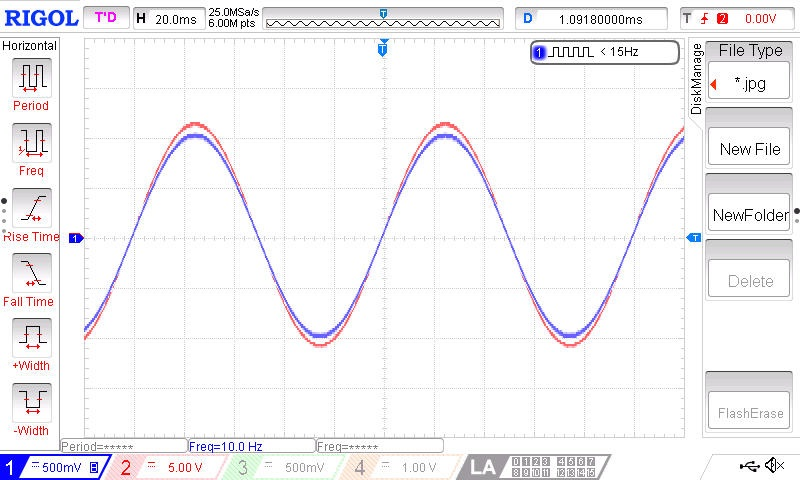
\includegraphics[width=\textwidth]{LAB/NewFile14.jpg}
    \end{minipage}
    \hfill
    \begin{minipage}[t]{0.49\textwidth}
      \(10\-[kHz]\), \(U_{ss-in} = 2.06\-[V]\), \(U_{ss-out} = 22.6\-[V]\)\\
      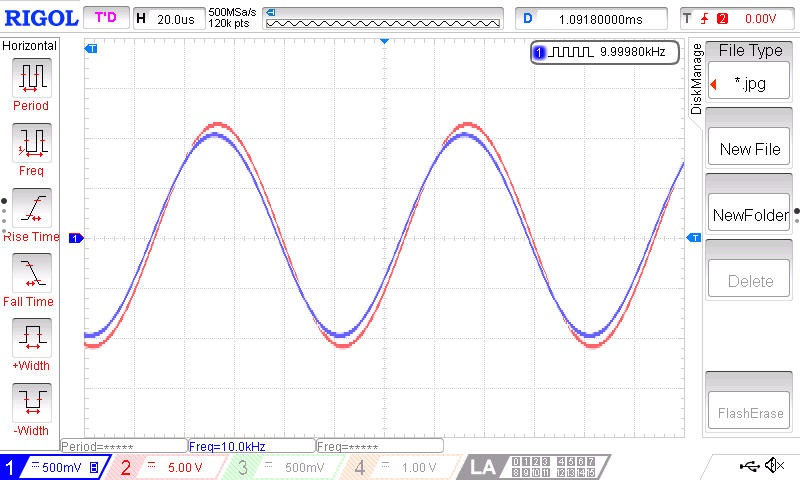
\includegraphics[width=\textwidth]{LAB/NewFile15.jpg}
    \end{minipage}
    \vspace{-4mm}
  \end{figure}
  \begin{figure}[H]
    \begin{minipage}[t]{0.49\textwidth}
      \(100\-[kHz]\), \(U_{ss-in} = 208\-[mV]\), \(U_{ss-out} = 1.82\-[V]\)\\
      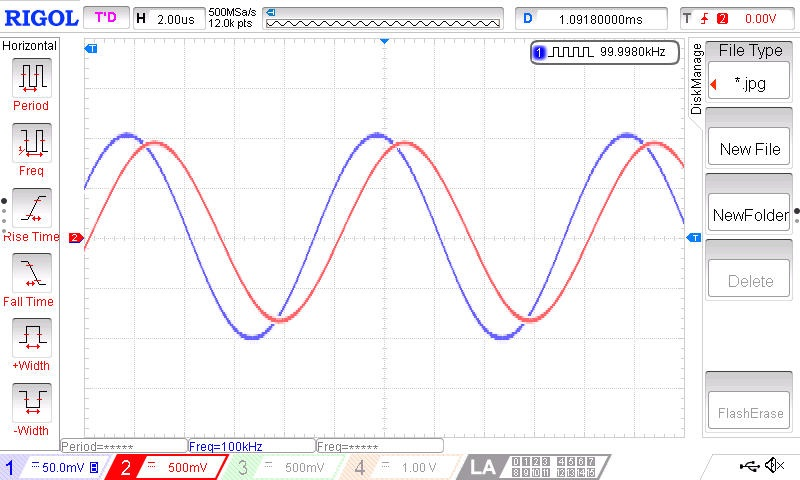
\includegraphics[width=\textwidth]{LAB/NewFile17.jpg}
    \end{minipage}
    \hfill
    \begin{minipage}[t]{0.49\textwidth}
      \(5\-[MHz]\), \(U_{ss-in} = 208\-[V]\), \(U_{ss-out} = 70\-[mV]\)\\
      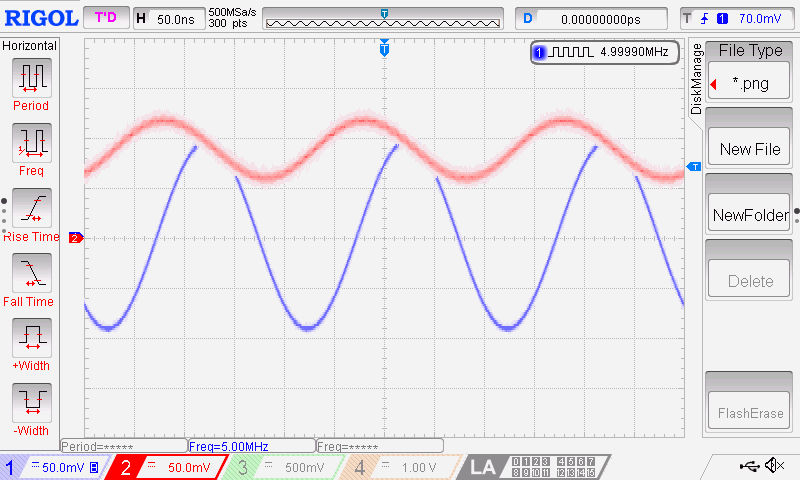
\includegraphics[width=\textwidth]{LAB/NewFile05.png}
    \end{minipage}
  \end{figure}
  \vspace{-2mm}
  \centering{\obrlabel{sin_prubehy}}
\end{figure}

\begin{minipage}[t]{\textwidth}
  \vspace{-7mm}
  \begin{tikzpicture}
    \begin{semilogxaxis}
      [
          width=1\textwidth, 
          height=75mm,
          title={Amplitudová kmitočtová charakteristika},
          xlabel={\(f\-[kHz]\)},
          ylabel={\(A\-[dB]\)},
          xmin=0.01, xmax=5000,
          ymin=-10, ymax=23,
          legend pos=south west,
      ]
      \addplot[
        color=blue,
        mark=x,
        ]
        coordinates {
          (0.01,  20.72761596 )
          (10  ,  20.80482438 )
          (100 ,  18.75704187 )
          (150 ,  17.19248586 )
          (200 ,  15.42404781 )
          (250 ,  13.89628089 )
          (300 ,  12.64046429 )
          (350 ,  11.39750616 )
          (400 ,  10.70226403 )
          (450 ,   9.679213585)
          (500 ,   8.519374645)
          (550 ,   7.252521338)
          (600 ,   6.503273508)
          (700 ,   5.242238593)
          (850 ,   3.766514309)
          (1000,   2.498774732)
          (1500,  -0.599264468)
          (5000,  -9.542425094)
        };
      \addlegendentry{\scriptsize \(C_v = 10\-[nF]\)}
      \addplot[
        color=red,
        mark=o,
        only marks,
        ]
        coordinates {
          (3000,  -3.039151587)
        };
      \addlegendentry{\scriptsize Pravděpodobně chybně změřený bod}
      \addplot[
        color=black,
        dotted,
        thick,
        mark=o,
        ]
        coordinates {
          (150 ,  17.19248586)
          (150 ,  -100)
        };
      \addplot[
          dotted,
          thick,
          color=black,
        ]
        coordinates {
          (0.01, 0)
          (5000, 0)
        };
        % \addlegendentry{\scriptsize \(C_v = 10\-[nF]\)}
    \end{semilogxaxis}
  \end{tikzpicture}
\end{minipage}

\begin{figure}[H]
  \centering
  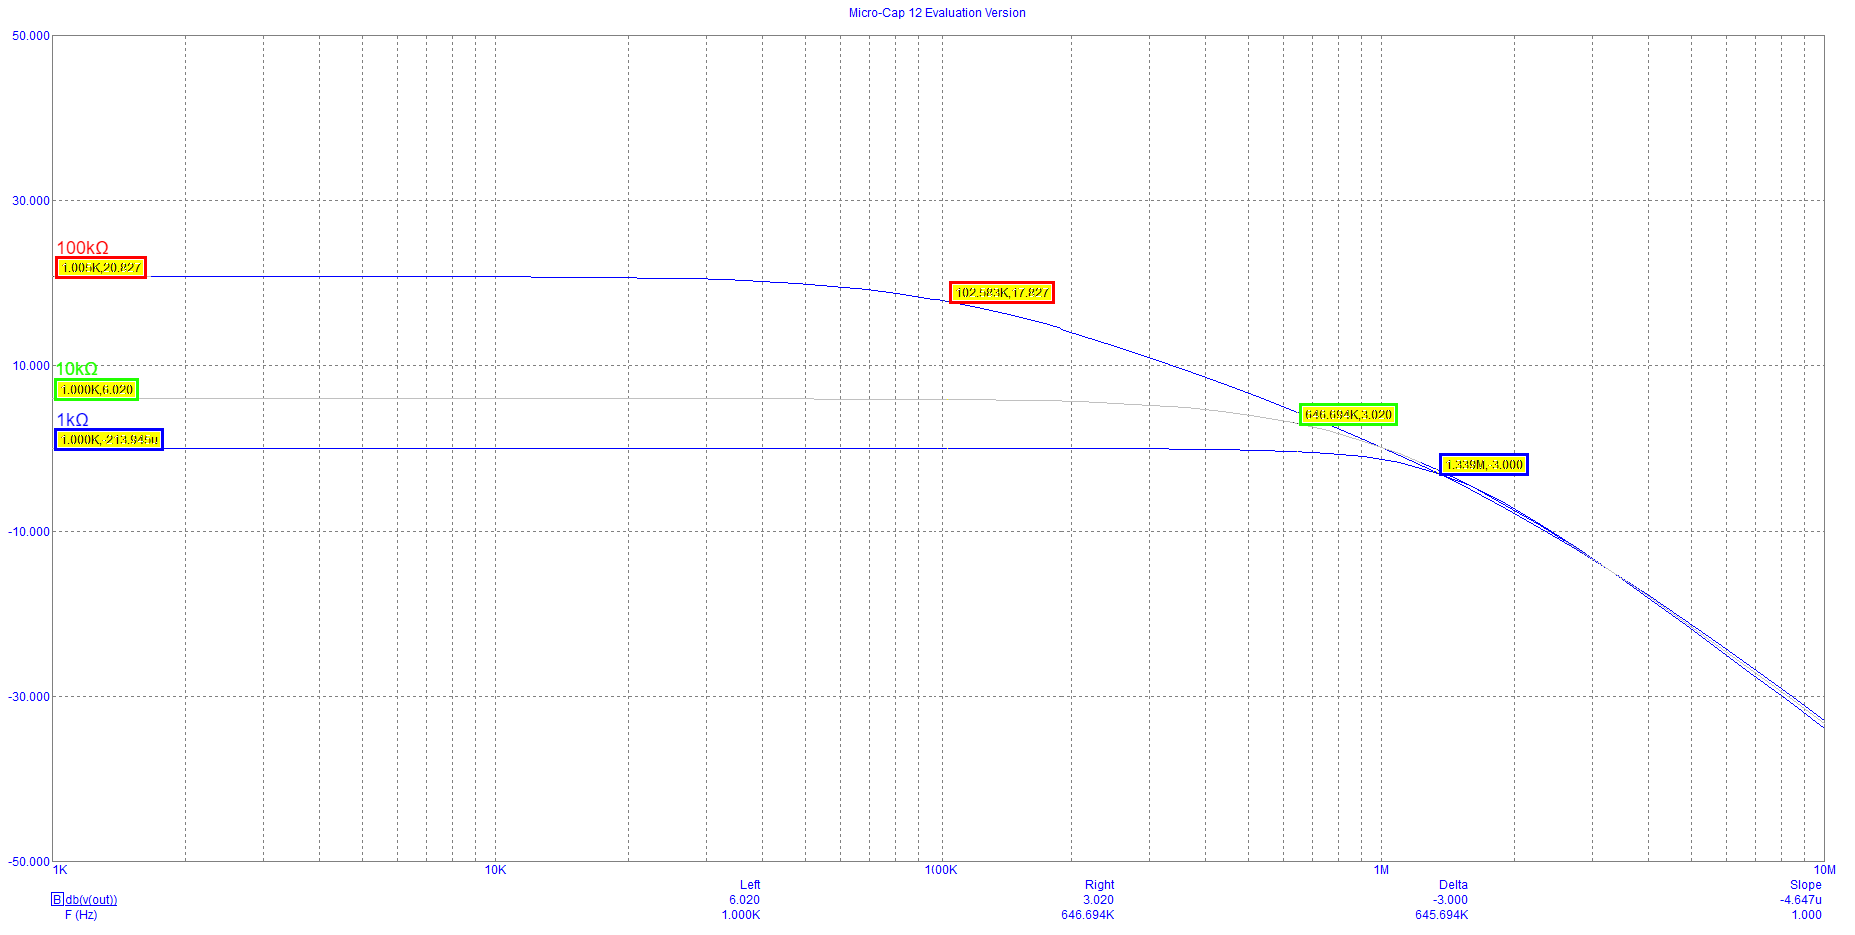
\includegraphics[width=0.8\textwidth]{PC/AC/nein_1k.png}
  \begin{center}
    Neinvertující zapojení OZ
  \end{center}
\end{figure}

\begin{figure}[H]
  \centering
  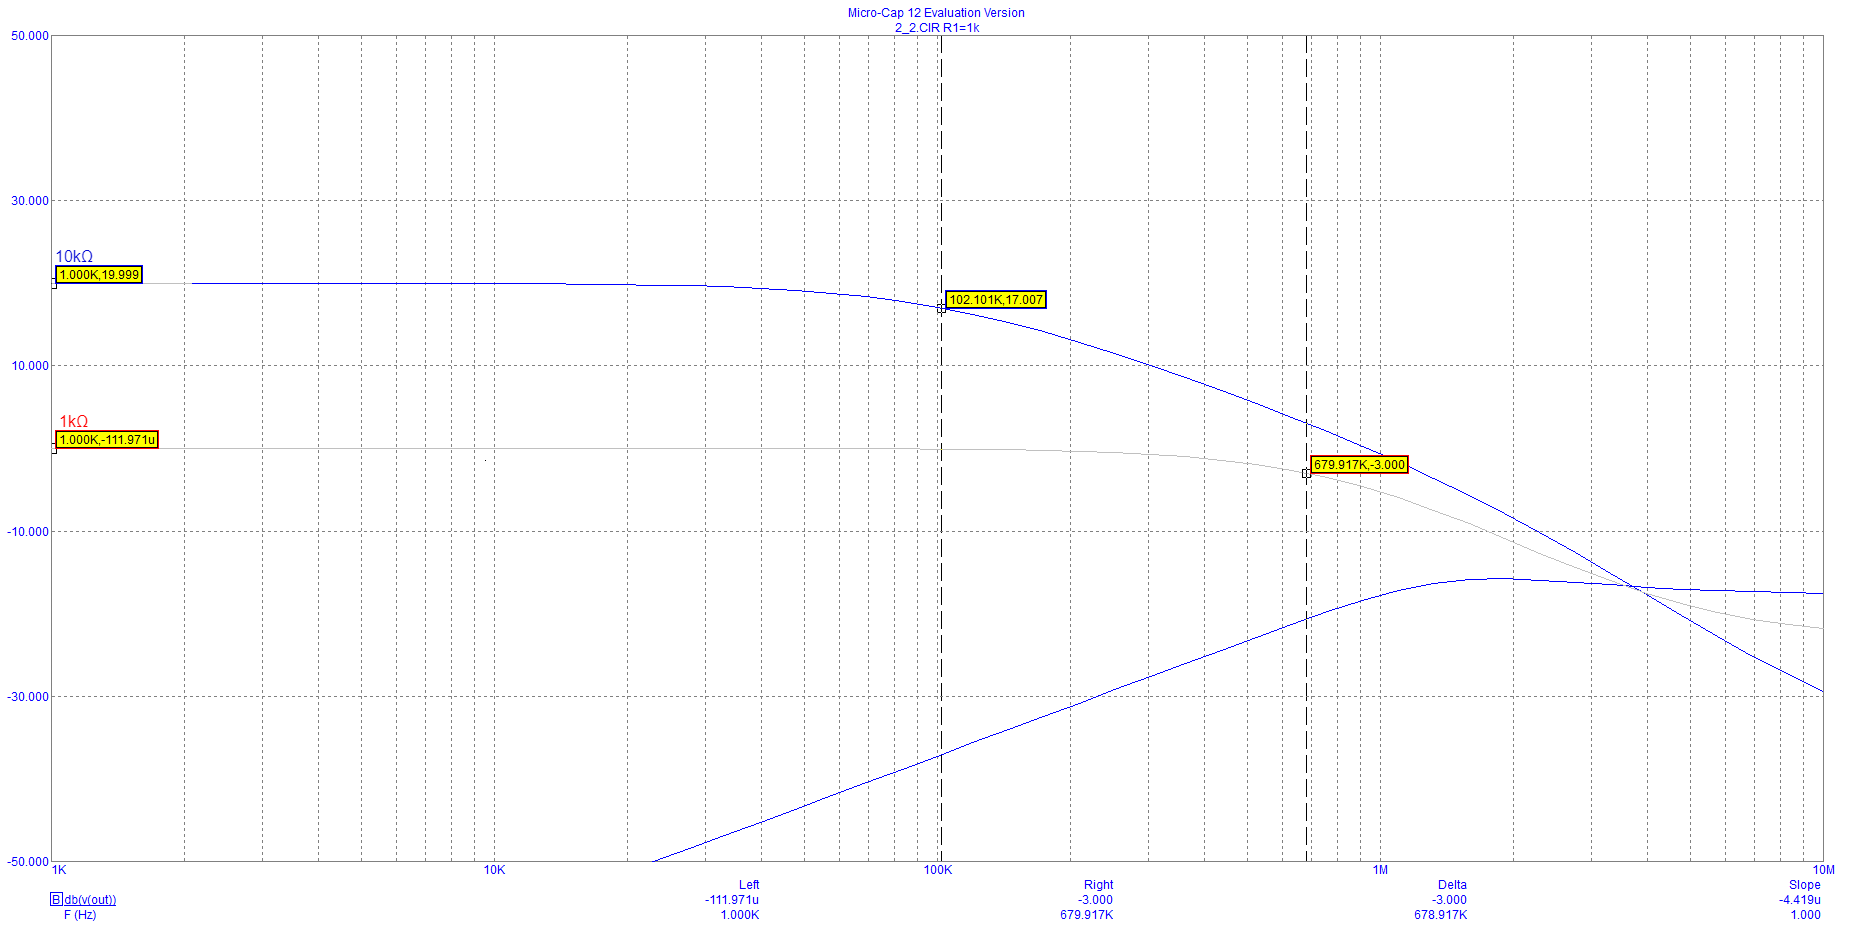
\includegraphics[width=0.8\textwidth]{PC/AC/in_1k.png}
  \begin{center}
    Invertující zapojení OZ
  \end{center}
\end{figure}

\subsection*{Napětová převodní charakteristika}
\begin{minipage}[t]{\textwidth}
  \(R_1 = 1,10,100\-[k\Omega]\)\\
  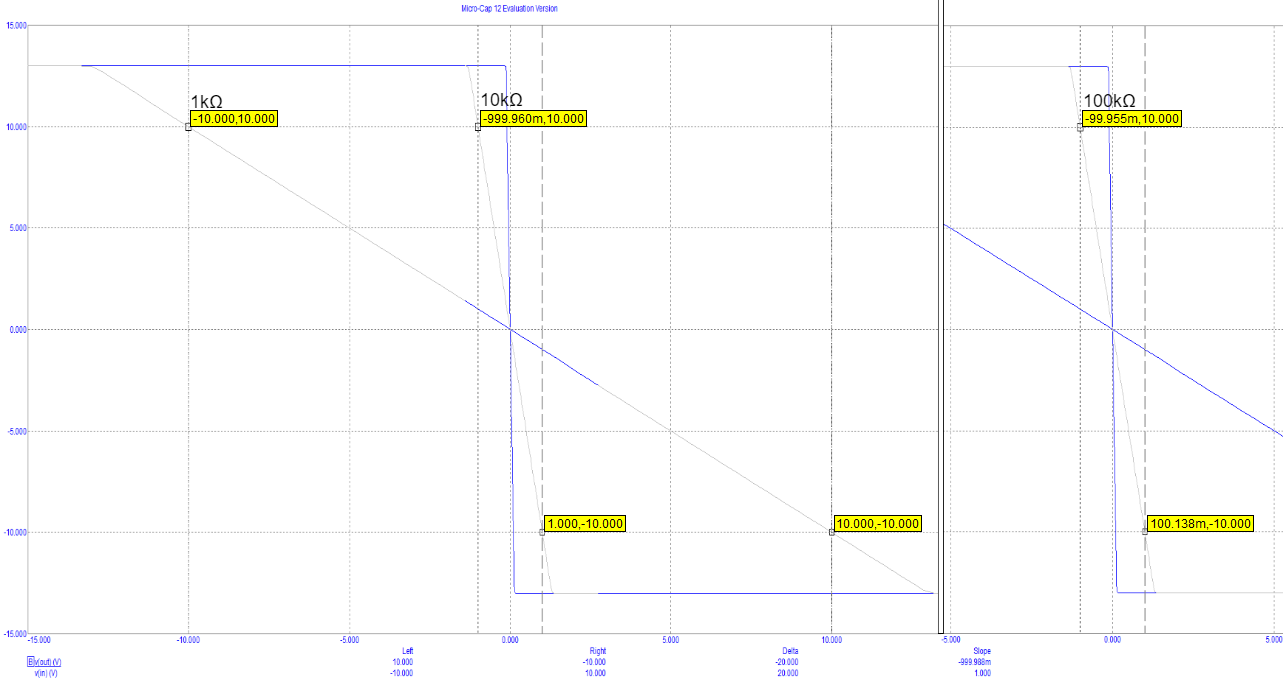
\includegraphics[width=\textwidth]{PC/DC/in_1k.png}
\end{minipage}
Mimo saturaci se zesílení v napětové převodní charakteristice projeví jako směrnice křivky.

\begin{figure}[H]
  \begin{figure}[H]
    \begin{minipage}[t]{0.49\textwidth}
      \(R_1 = 1\-[k\Omega]\)\\
      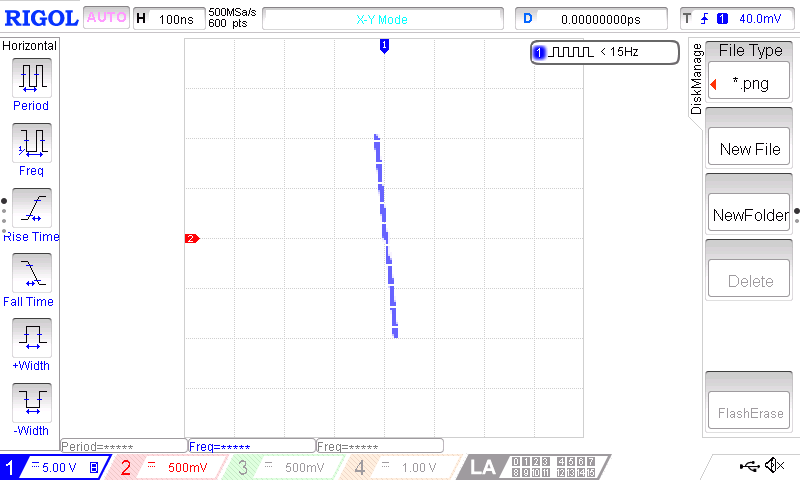
\includegraphics[width=\textwidth]{LAB/NewFile14.png}
    \end{minipage}
    \hfill
    \begin{minipage}[t]{0.49\textwidth}
      \(R_1 = 10\-[k\Omega]\)\\
      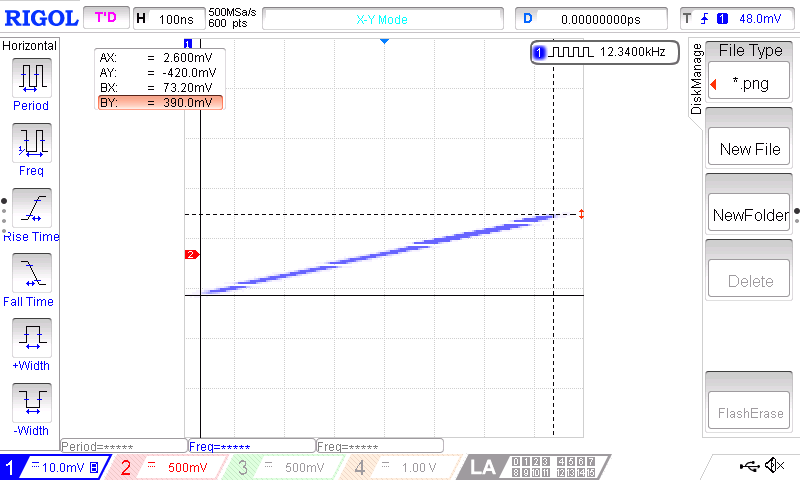
\includegraphics[width=\textwidth]{LAB/NewFile06.png}
    \end{minipage}
    \vspace{-4mm}
  \end{figure}
\end{figure}

\begin{figure}[H]
  \centering
  \(R_1 = 100\-[k\Omega]\)\\
  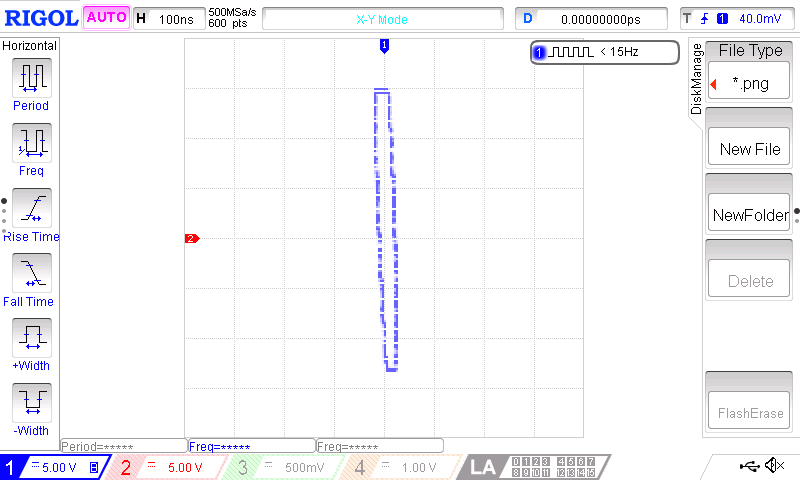
\includegraphics[width=0.5\textwidth]{LAB/NewFile13.png}
\end{figure}

\subsection{Závěr}

\begin{table}[H]
  % \centering
  \begin{tabular}{|c|c|c|} 
    \hline
    -               & \(SR_{up}\-[V/\mu s]\)  & \(SR_{down}\-[V/\mu s]\) \\ \hline
    simulace        & 0.5591                  & 0.5533                   \\ \hline
    měření          & 0.9947                  & 0.8144                   \\\hline
  \end{tabular}
  \normalsize
  \caption{\label{tab_pracovni_bod_rozladeni1}}
\end{table}

Při měření mezní rychlosti přeběhu jsme došli ke čtyřem výsledkům (ze simulace a z reálného měření).
Ze simulace vychází \(RS_{up} = 0.5591\-[V/\mu s], RS_{down} = 0.5533\-[V/\mu s]\).
Zatím co z reálného měření vyšlo \(RS_{up} = 0.9947\-[V/\mu s], RS_{down} = 0.8144\-[V/\mu s]\).
Vzhledem k velké odchylce jsem nahlédl do datasheet OZ 1458 \\(www.st.com/resource/en/datasheet/mc1458.pdf strana 6), kde je typická rychlost přeběhu při napájení \(\pm 10\-[V]\) \(SR = 0.8\-[V/\mu s]\), minimální \(0.2\-[V/\mu s]\) a maximální není uvedena.
Předpokládám proto, že Simulace počítala s modelem, který je podle datasheetu sice možný, ale ne úplně typický.
% Při měření bylo napájecí napětí \(\pm 15\-[V]\) namísto \(\pm 10\-[V]\) jako v datasheet byla hodnota \(SR\) možná o něco vyšší.

Reálné průběhy na straně 3.
Na obrázku \(A\) i \(B\) je zobrazen vstupní a výstupní signál stejného zapojení se stejnou frekvencí \(f = 1\-{kHz}\) ale jinou amplitudou vstupního resp. výstupního signálu. 
Pokud by nedošlo k saturaci, tak by zesílení \(A\) mělo být u obou průběhů stejně \(A = 13.59\-[V]\).
Na obrázku \(B\) však dochází k saturaci a signál je tak omezen na napětí v intervalu \(\pm 14.3\-[V]\).

Při měření frekvenčního rozsahu (strana 4 obr. 1) je vidět, jak se se vzrůstající frekvencí snižuje zesílení a posouvá fáze.
Navíc je při frekvencích nad 1\-{kHz} vidět, že se k výstupnímu signálu přidává stejnosměrná složka, která je pravděpodobně způsobena asymetrií výstupu zesilovače.
Na grafu závislosti zesílení na frekvenci je vidět, že první měření, které je oproti maximu sníženo o \(3\-[dB]\), je na frekvenci \(150\-{kHz}\).

Při simulaci invertujícího zapojení s odporem \(R_1 = 100\-[k\Omega]\) je jasně vidět chyba simulátoru.
Tato chyba způsobuje, že zapojení, které by mělo mít při nulové frekvenci zesílení \(A = 40\-[dB]\), má zesílení hluboko v záporných číslech.
Tato chyba je však viditelná i u druhých dvou průběhů, kde se viditelně projevuje na vysokých frekvencích.

Mimo saturaci se zesílení v napěťové převodní charakteristice zobrazí jako směrnice, v simulaci je to zřetelně viditelné.
V našem reálném měření je směrnice sice viditelná také, ale je velmi nepřesná.

\end{document}
